\subsection{Continued free institutional redesign under different losses}
\label{sec:native-objective-redesign-v12}

This finite slice combines the earlier objective-conditioned structural
question with a broader externally authored redesign path. V11's generic
interface is open, but its empirical vocabulary deliberately retains two
aggregation algorithms and a cutoff. V12 instead requests a complete executable
vocabulary at every generation: Python algorithms, mechanisms, protocols,
connections and activity processes can change, or be retained in light of the
arm's own history. Renaming a node or changing a hash alone is not institutional
invention. The original researcher/project/paper/retrieval/resource world and
fixed researcher weights remain the forward environment.

The prospectively fixed main budget is two exact existing objectives---throughput
$-A$ and reviewed utility $3.25A-Q+.05R$---by three sequential generations and
one design draw per generation, six native attempts maximum. The initial
system, five authors, two years, development seed 42 and four-year real-paper
corpus are held fixed. Derivative-free external redesign sees only its own
preceding source, losses and failures. This is not a claimed Bayesian optimizer,
a gradient of arbitrary source invention or a causal comparison across
independent seeds. No hidden quality/fairness veto or novelty reward is used.
The opt-in singleton black-box path records an observation and does not compute
a leave-one-out score estimate; score/hybrid batches still require two draws.

A separately bound two-world forward-only followup tests V11's final saved
corrected-control proposal distribution, rather than appending trials to that
closed campaign. Its draw stream is 43 while scientific seed 42 remains unchanged.
The parent audit, vocabulary, final weights and original runtime continuity are
checked before inference; the narrowly reviewed optimizer extension is recorded.
No further optimizer update is performed, and two observations cannot establish variance
reduction, optimizer advantage or beneficial science policy.

Every completed main checkpoint is cross-scored under both declared losses
afterward. These are the same development worlds, not held-out replications or
an extra selection objective. Native receipts must distinguish installed source,
actual source execution, information delivery and committed effects. All
unsuccessful, null and tied observations remain visible. The eight-attempt
combined budget is fixed before results, not extended until an improvement
appears.

\paragraph{Main native results and paths.}
All six main worlds complete at clean source \code{ecab4b4}, with 565 fresh
Qwen replies, no response reuse and no world-level technical failure.
Table~\ref{tab:free-redesign-v12} shows every outcome in both objective
coordinates; Figure~\ref{fig:free-redesign-v12} separates current proposals
from their retained best. The throughput path is $[-10,-10,-10]$; utility is
$[-1/6,0,-1/6]$ up to floating-point representation. Both arms select their G0
institution, with three and two exact best-loss observations respectively.
Repeated outcomes at one scientific seed are separate physical executions,
not independent replications or additional evidence of generalization.

\begin{table}[t]
\centering\small
\caption{Every main development outcome, cross-scored from the same native
checkpoint. Graph is nodes/wires. $Q$ uses original reviewer means, not
institution-authored final scores; displayed decimals are rounded.
No initial-system score or held-out result is fabricated.}
\label{tab:free-redesign-v12}
\begin{tabular}{llrrrrr}
\toprule
Arm/generation & Graph & $A$ & $Q$ & $R$ & Count loss & Utility loss \\
\midrule
Throughput G0 & 17/25 & 10 & 31.667 & 30 & $-10$ & 2.3333 \\
Throughput G1 & 17/25 & 10 & 31.667 & 30 & $-10$ & 2.3333 \\
Throughput G2 & 17/25 & 10 & 31.667 & 30 & $-10$ & 2.3333 \\
\addlinespace[3pt]
Utility G0 & 16/22 & 3 & 10.667 & 15 & $-3$ & $-.1667$ \\
Utility G1 & 17/24 & 1 & 4 & 15 & $-1$ & 0 \\
Utility G2 & 16/22 & 3 & 10.667 & 15 & $-3$ & $-.1667$ \\
\bottomrule
\end{tabular}
\end{table}

\paragraph{What actually changed.}
The throughput author installs a production office that shares real earlier
papers, an annual-sprint scheduler that emits typed native plan amendments,
and admission code accepting actual submissions. Ten amendments per world
scope native projects to annual completion and submission; the world records
five accepted decisions per year, ten across two years. Later generations
retain the exact executable institution after their own observations.
This saturates the observed ordinary one-lead-paper-per-author-year workflow,
not the unrestricted representational design space or a global optimum.

The utility author instead installs an evidence office and uses original
reviewer mean greater than 3.25 for admission. Holding reviewer scores and later
outcomes fixed, admission changes the loss contribution by $3.25-q$. The
threshold is a loss-derived greedy rule, not a hidden quality constraint or an
optimal policy for the full world. In G1 it adds a milestone-clinic source node, typed amendment
transport and two wires, while revising evidence-topic matching. The intended
two-year research cycle produces two actual plan amendments and a completed
native world, but loss worsens from $-1/6$ to zero without reducing $R=15$.
G2 therefore retains the exact G0 incumbent. Its parent is G0, not the worse
chronological G1; zero changes against that parent do not conceal the rejected
revision. Scripted six-year technical QA counts are not actual-Qwen effects.

The selected institutions differ in source, graph, activity timing and
admission rule, with different cross-objective profiles. However, neither
improves its first native observation. These results demonstrate an executable
loss-conditioned redesign/execute/measure/retain loop, not successful adaptive
invention, an improved designer, optimizer efficiency or a causal objective
effect. External Codex authorship is self-reported and own-history access is
an instruction/request contract, not operating-system isolation or provider
authentication. Native receipts establish execution and committed effects;
they do not identify which simultaneous edit caused a loss difference or
whether a delivered message improved science.
The independent audit preserves all 107 raw files and repeated reports are
byte-identical. It verifies 32 committed source executions and the amendment
commands against source outputs, event/wire lineage and annual actor state.
The recorded code ABI does not retain a fully bound upstream-plan context,
so reconstructing the complete applied-plan hash is unavailable in this
actual slice; that stronger proof is not claimed. Accumulated measured
model-call time is 2166.53 seconds (36.11 minutes), not overall wall time.

\begin{figure}[p]
\centering
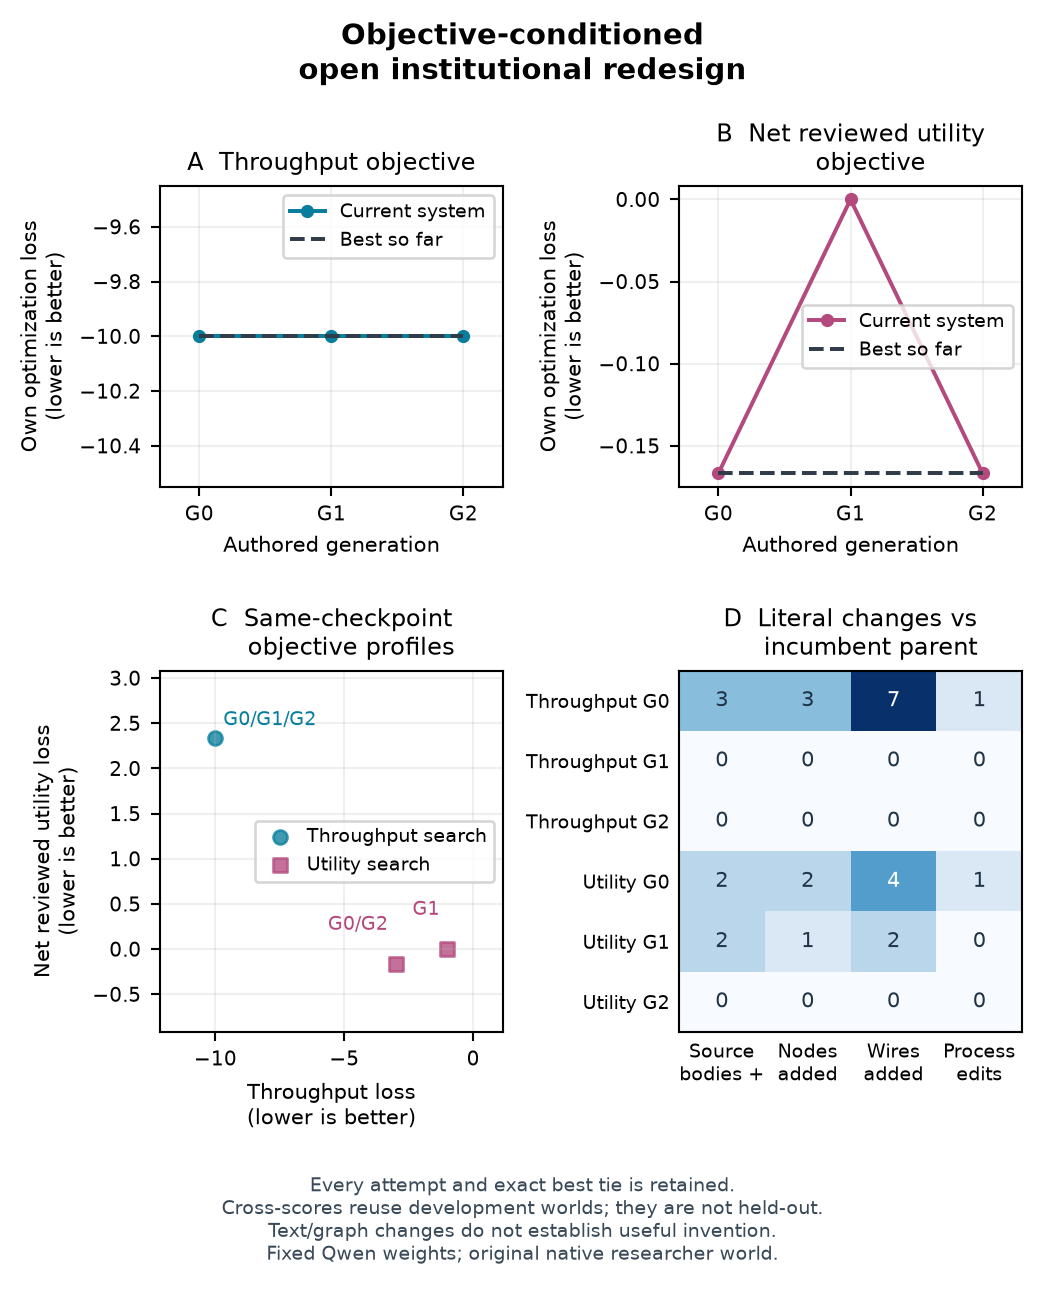
\includegraphics[width=\linewidth]{figures/native-objective-redesign-v12-a1.png}
\caption{Audited free-redesign development paths. A/B use separate own-loss
scales and distinguish current from retained best. C reuses each checkpoint
under both losses, not held-out data. D counts literal executable changes
against the request's incumbent parent, not the previous chronological draw;
G2 utility returns to G0. Source counts are not semantic novelty or scientific
benefit. Every outcome and exact tie remains visible.}
\label{fig:free-redesign-v12}
\end{figure}

\paragraph{Separate final-control forward result.}
The two followup worlds both complete at clean source \code{ecab4b4}, using
180 fresh Qwen replies with no replay or world-level technical failure.
Table~\ref{tab:final-control-followup-v12} reports the complete fixed budget.
An independent audit re-extracts the native losses, reconstructs the final
proposal and draws, and re-audits the original v11 parent (actual source
\code{acf3a2e}) using clean historical audit source \code{77e3b9e}. These sources
are distinct and their relevant native runtime blobs are checked.
Repeated audits are byte-identical and leave all 32 followup
raw files and the archived parent unchanged. Accumulated measured model-call
time is 658.63 seconds (10.98 minutes), not overall wall time.

This supplies the previously missing forward evaluations of the final saved
control-update distribution. It does not show that the control variate lowers
expected loss or estimator variance. Historical v11 outcomes are provenance,
not a concurrent control group; the two new outcomes do not establish causal
improvement, a reliable expectation or scientific value.

\begin{table}[t]
\centering
\caption{All fresh native outcomes from the final v11 saved proposal. The cutoff
is the actual bounded consumer value, not the Gaussian latent. Original review
records determine $A,Q,R$ and the unchanged utility loss.}
\label{tab:final-control-followup-v12}
\begin{tabular}{lrrrrrr}
\toprule
Aggregation & Cutoff & $A$ & $Q$ & $R$ & Loss & Replies \\
\midrule
Minimum & 3.549508 & 0 & 0 & 21 & 1.05 & 91 \\
Mean & 3.080488 & 2 & 7 & 21 & .55 & 89 \\
\bottomrule
\end{tabular}
\end{table}
